\section{Descripción de procesos}

El sistema operativo administra la ejecución de los procesos y los recursos del sistema. Para ello planifica la utilización del procesador, asigna memoria y dispositivos de E/S, administra archivos y responde a las solicitudes realizadas por los procesos. En esencia, puede considerarse como el encargado de gestionar todos los recursos del sistema.

\begin{figure}[!ht]
  \centering
  \includegraphics[width=0.7\linewidth]{chapters/02_unit/media/proceses_and_resources.pdf}
  \caption{Recursos y procesos.}
\end{figure}

En un entorno multiprogramado existen múltiples procesos que compiten por dichos recursos. Mientras algunos se encuentran ejecutándose, otros pueden estar bloqueados esperando una operación de E/S o suspendidos por falta de memoria. Para poder coordinar estas situaciones, el sistema operativo debe mantener información actualizada sobre el estado de cada proceso y de cada recurso.

\subsection{Estructuras de control del sistema operativo}

La forma habitual de organizar esta información consiste en mantener un conjunto de tablas de control, como se ilustra en la figura \ref{fig:os_tables}, cada una dedicada a un tipo de recurso. De forma general, un sistema operativo mantiene cuatro categorías de tablas:
\begin{itemize}
  \item Tablas de memoria: registran la asignación de memoria principal y secundaria, los mecanismos de memoria virtual y los atributos de protección de cada región.
  \item Tablas de E/S: almacenan el estado de los dispositivos, las operaciones de entrada/salida en curso y los procesos que utilizan cada dispositivo.
  \item Tablas de archivos: contienen información sobre los archivos del sistema, como su ubicación, estado y atributos.
  \item Tablas de procesos: mantienen toda la información necesaria para administrar cada proceso, constituyendo la estructura de datos más importante para el planificador.
\end{itemize}
\begin{figure}[!ht]
  \centering
  \includegraphics[width=0.9\linewidth]{chapters/02_unit/media/os_tables.pdf}
  \caption{Estructura general de las tablas del Sistema Operativo.}
  \label{fig:os_tables}
\end{figure}

Estas tablas no son independientes, sino que se encuentran relacionadas entre sí. Un proceso referencia regiones de memoria, dispositivos de E/S y archivos; de igual forma, los archivos residen en dispositivos de almacenamiento y las propias tablas deben almacenarse en memoria. Por ello, el sistema operativo mantiene referencias cruzadas entre todas estas estructuras para administrar de forma coherente los recursos del sistema.

Durante la inicialización del sistema, el sistema operativo construye estas tablas a partir de la información de configuración del hardware, como la cantidad de memoria disponible y los dispositivos presentes en el sistema.

\subsection{Estructuras de control de procesos}

Para administrar un proceso, el sistema operativo debe conocer dos aspectos fundamentales:
\begin{enumerate}
  \item dónde se encuentra el proceso en memoria;
  \item cuál es su estado y el resto de la información necesaria para administrarlo.
\end{enumerate}

\subsubsection{Ubicación e Imagen del Proceso}

Un programa en disco es una entidad pasiva. Un proceso es una entidad activa que el SO debe poder pausar, mover y reanudar. Para ello, el SO mantiene para cada proceso su \emph{imagen del proceso}: representación concreta y completa de ese proceso en un instante dado.

La imagen del proceso se compone de:
\begin{itemize}
  \item Código: las instrucciones del programa.
  \item Datos: variables globales, heap y datos del programa.
  \item Pila: pila de usuario para llamadas a funciones y pila de kernel para llamadas al sistema.
  \item Bloque de control (PCB): estado, contador de programa, registros y, fundamentalmente, los punteros que indican dónde se encuentra cada una de las regiones anteriores.
\end{itemize}

\begin{figure}[!ht]
  \centering
  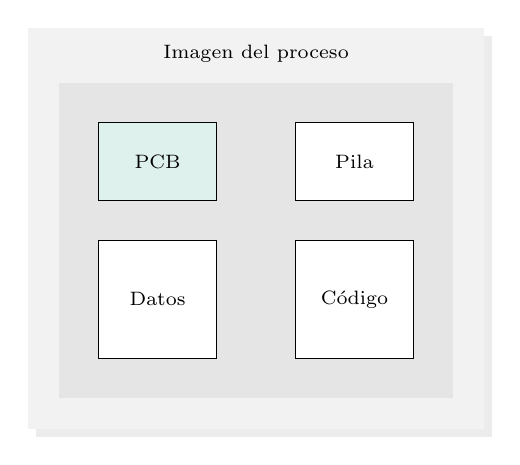
\begin{tikzpicture}[font=\scriptsize]
    \fill[gray!15] (-.3,-.5) rectangle (5.5,4.6);
    \fill[gray!10] (-.4,-.4) rectangle (5.4,4.7);
    \node[below,align=center] at(2.5,4.6) {Imagen del proceso};
    \fill[gray!20] (0,0) rectangle (5,4);
    \draw[fill=white!94!blue!93!green] (0.5,2.5) rectangle node[text width=1.5cm,align=center]{PCB} (2,3.5);
    \draw[fill=white] (0.5,0.5) rectangle node[text width=1.5cm,align=center]{Datos} (2,2);
    \draw[fill=white] (3,2.5) rectangle node[text width=1.5cm,align=center]{Pila} (4.5,3.5);
    \draw[fill=white] (3,0.5) rectangle node[text width=1.5cm,align=center]{Código} (4.5,2);
  \end{tikzpicture}
  \caption{Estructura lógica de la imagen de un proceso. Físicamente, el PCB reside en memoria del kernel siempre en memoria principal, mientras que el resto de las regiones puede estar disperso.}
\end{figure}

La imagen del proceso puede no estar completamente en memoria principal en un instante dado\footnote{En el capítulo \ref{chpt:memoria} se estudiará en detalle el mecanismo de memoria virtual que hace esto posible, permitiendo mantener en memoria principal solo las partes necesarias en cada momento.}. Por este motivo, el PCB cumple el rol de \emph{descriptor central}, contiene la información necesaria para reconstruir la imagen.

En particular, guarda dónde se encuentra cada región de la imagen ---por ejemplo, las regiones de código, datos y pila--- y los punteros hacia las estructuras que describen el resto de los recursos asignados, como los archivos abiertos.

En consecuencia, el SO no necesita conocer de antemano dónde está cada parte de la imagen: le basta con encontrar el PCB, y desde él puede localizar todo lo demás. El PCB es, por definición, la única parte que permite acceder a todas las demás.

¿Cómo encuentra el sistema operativo al PCB? Este es el aspecto fundamental del mecanismo de control. A diferencia del resto de la imagen, que puede estar paginada y dispersa, el PCB tiene una ubicación privilegiada y siempre accesible. El PCB no se almacena en el espacio de usuario del proceso. Se almacena en el espacio de memoria del propio kernel, en una región \emph{residente y contigua}. El sistema operativo mantiene el acceso al PCB de cada proceso existente en las tablas de procesos (Figura \ref{fig:os_tables}).

Para encontrar un PCB específico, el sistema operativo puede proceder mediante dos vías:
\begin{enumerate}
  \item Proceso en ejecución: El kernel mantiene un puntero global, usualmente denominado \texttt{current} o \texttt{running}, que apunta siempre al PCB del proceso que actualmente posee la CPU. Ante una interrupción, llamada al sistema o excepción, el hardware transfiere el control al kernel, y este ya conoce el PCB actual sin necesidad de búsqueda.
  \item Cualquier otro proceso: Para localizar un proceso diferente (por ejemplo, para planificarlo o enviarle una señal), el SO utiliza su identificador único (\emph{PID}). El PID actúa como índice o clave de búsqueda en la Tabla de Procesos, lo que devuelve inmediatamente la dirección del PCB correspondiente.
\end{enumerate}
El PCB es la única estructura que el sistema operativo necesita encontrar directamente; una vez hallado, toda la imagen del proceso se vuelve localizable.

\subsubsection{Atributos del proceso}

Aunque la organización exacta del PCB depende de cada sistema operativo, su contenido responde siempre a tres funciones distintas. Esta es la clasificación que ya se adelantó al presentar el concepto de proceso, ahora ilustrada en la figura \ref{fig:process_struct}.

\begin{enumerate}
  \item \textbf{Identificación:} permite al SO distinguir al proceso y relacionarlo con otras estructuras. Incluye el identificador único (PID), el usuario propietario y las relaciones de parentesco.
  \item \textbf{Estado del procesador:} es el contexto mínimo para poder pausar y reanudar. Incluye el contador de programa (PC), los registros de propósito general, los punteros de pila y el \emph{Program Status Word} (PSW).
  \item \textbf{Información de control:} es todo lo que el SO necesita para administrarlo: estado de planificación, prioridad, recursos asignados como memoria y archivos abiertos, y enlaces con otros PCB.
\end{enumerate}

\begin{figure}[!ht]
  \centering
  \includegraphics[width=0.8\textwidth]{chapters/02_unit/media/process_struct.pdf}
  \caption{Contenido típico del PCB agrupado según su función.}
  \label{fig:process_struct}
\end{figure}

Esta estructura conceptual se materializa de forma muy diferente según el sistema operativo.

En Linux, el PCB se implementa como \texttt{task\_struct}, que puede ser consultado a continuación.

\url{https://elixir.bootlin.com/linux/latest/source/include/linux/sched.h}

Si se consulta su definición en el código fuente se puede ver que es una estructura grande, en torno a 8KB y con más de 150 campos según la versión del kernel, que agrupa las tres categorías: identificación con \texttt{pid} y \texttt{tgid}, estado del procesador con \texttt{thread\_struct}, e información de control con \texttt{mm\_struct}, \texttt{files\_struct} y \texttt{cred}.

De hecho, al ser una estructura en memoria del kernel, es posible inspeccionarla en vivo. En la documentación oficial se muestra el caso del proceso \texttt{init} en una máquina virtual, donde mediante un debugger se modifica su campo \texttt{comm} para cambiarle el nombre en tiempo de ejecución. Es una demostración muy clara de que el PCB es una estructura de datos manipulable:

\url{https://linux-kernel-labs.github.io/refs/heads/master/lectures/processes.html}

En Windows, el equivalente es la estructura \texttt{EPROCESS}, perteneciente al ejecutivo del kernel. Aunque está parcialmente indocumentada, Microsoft expone su rol y sus campos principales en la documentación de drivers:

\url{https://learn.microsoft.com/en-us/windows-hardware/drivers/kernel/eprocess}

En ambos casos se observa la misma idea: el PCB concentra toda la información que el SO necesita. Por eso prácticamente todos los módulos ---planificador, administrador de memoria, E/S--- interactúan con él y su acceso debe estar protegido. Una corrupción en esta única estructura compromete toda la administración del proceso.

\section{Control de procesos}

\subsection{Modos de ejecución}

Para garantizar la protección del sistema, la mayoría de los procesadores implementan al menos dos modos de ejecución:
\begin{itemize}
  \item Modo usuario (\emph{user mode)}: utilizado por las aplicaciones. En este modo no es posible ejecutar instrucciones privilegiadas ni acceder directamente a recursos críticos del sistema.
  \item Modo kernel (\emph{kernel mode)}: utilizado por el sistema operativo. Proporciona acceso completo al procesador, la memoria y los dispositivos de E/S, permitiendo ejecutar instrucciones privilegiadas.
\end{itemize}

La existencia de estos modos evita que un programa de usuario pueda modificar estructuras críticas del sistema operativo, como los PCBs, alterar registros de control o acceder libremente al hardware.

El modo de ejecución suele almacenarse en un bit (o conjunto de bits) del \emph{Program Status Word} (PSW).

\subsection{Creación de procesos}

Cuando el SO decide crear un nuevo proceso (cualquiera sea el motivo; ver sección \ref{ssec_creac_y_fin_procesos}), sigue estos pasos:
\begin{enumerate}
  \item Asignar un identificador único (PID) al proceso y agregar una nueva entrada en la tabla primaria de procesos.
  \item Asignar espacio para todos los elementos de la imagen del proceso: espacio de direcciones privado (programa y datos), pila de usuario, y el PCB.
  Estos tamaños pueden fijarse por defecto, por solicitud del usuario, o ser pasados por el proceso padre si este generó al nuevo proceso. Si va a compartir espacio de direcciones existente, se configuran los enlaces correspondientes.
  \item Inicializar el PCB:
  \begin{itemize}
    \item \emph{Identificación:} ID propio (y, de ser necesario, del proceso padre).
    \item \emph{Estado del procesador:} casi todo en cero, salvo el contador de programa (apunta al punto de entrada) y los punteros de pila del sistema.
    \item \emph{Control del proceso:} valores por defecto más los atributos solicitados. Por ejemplo, el estado inicial suele ser Listo o Listo/Susp; la prioridad, la más baja salvo que se pida otra explícitamente; y no posee recursos (E/S, archivos) salvo que se soliciten o se hereden del padre.
  \end{itemize}

  \item Fijar los enlaces correspondientes, por ejemplo, insertar el proceso en la lista enlazada de la cola de Listos o Listo/Susp.

  \item Crear o expandir otras estructuras de datos, como un archivo de contabilidad por proceso, usado luego para métricas o evaluación de rendimiento.
\end{enumerate}

\subsection{Conmutación de Procesos}

El cambio o conmutación de procesos ocurre cuando el sistema operativo obtiene el control del procesador y decide reemplazar el proceso en ejecución por otro. Este cambio implica actualizar el estado de los procesos y restaurar el contexto del nuevo proceso seleccionado.

\paragraph{Eventos que provocan un cambio de proceso}
Un cambio de proceso solo puede ocurrir cuando el sistema operativo toma el control del procesador. Las causas más comunes son:
\begin{itemize}
  \item Interrupciones (interrupts): eventos externos al proceso, como la finalización de una operación de E/S o la expiración del quantum. El sistema operativo decide si reanudar el proceso actual o despachar otro.
  \item Excepciones (traps): errores generados por el propio proceso (por ejemplo, acceso ilegal a memoria). Si la excepción es fatal, el proceso finaliza; en caso contrario, el sistema operativo puede intentar recuperarlo o reanudar su ejecución.
  \item Llamadas al sistema (system calls): solicitudes explícitas de un proceso al sistema operativo. Algunas operaciones, como una petición de E/S, pueden bloquear el proceso hasta que el recurso esté disponible.
\end{itemize}

Para poder realizar un cambio de proceso, se deben realizar dos acciones:
\begin{enumerate}
  \item Cambiar de modo,
  \item Realizar las operaciones de cambio de proceso.
\end{enumerate}

\paragraph{Cambio de modo}
El cambio de modo consiste en el cambio del procesador de \textit{user mode} a \textit{kernel mode}, generalmente como consecuencia de una interrupción, excepción o llamada al sistema. Durante este cambio:
\begin{enumerate}
  \item Se guarda el contexto del procesador (PC, registros y pila).
  \item El procesador entra en modo kernel.
  \item Se ejecuta el manejador correspondiente.
\end{enumerate}
El cambio de modo no implica necesariamente un cambio de proceso. Si el proceso interrumpido continúa ejecutándose tras finalizar el manejador, basta con restaurar el contexto previamente almacenado.

\paragraph{Cambio de proceso}
Si el sistema operativo decide reemplazar el proceso en ejecución, además del cambio de modo (los tres pasos anteriores) debe realizar un cambio de proceso. Este procedimiento comprende:
\begin{enumerate}
  \item Guardar el contexto del proceso actual.
  \item Actualizar su PCB, incluyendo su nuevo estado (\textit{Ready}, \textit{Blocked}, \textit{Exit}, etc.).
  \item Mover el PCB a la cola correspondiente.
  \item Ejecutar el planificador para seleccionar un nuevo proceso para ejecutar.
  \item Actualizar el PCB del proceso seleccionado, cambiando su estado a \textit{Running}.
  \item Actualizar la unidad de gestión de memoria (MMU/TLB) cargando los punteros de la tabla de páginas del nuevo proceso (esto es muy costoso en tiempo computacional).
  \item Restaurar el contexto del nuevo proceso.
\end{enumerate}
El cambio de proceso tiene un costo mayor que un cambio de modo, ya que además de guardar y restaurar el contexto requiere modificar los estados de los procesos y las estructuras internas del sistema operativo.

\section{Modelos de Ejecución del SO}

Aunque el sistema operativo es un conjunto de programas ejecutados por el procesador, existen distintas estrategias para organizar su ejecución. Estas difieren principalmente en cómo se relaciona el código del kernel con los procesos de usuario.

\begin{figure}[!ht]
  \centering
  \begin{subfigure}[c]{\linewidth}
    \centering
    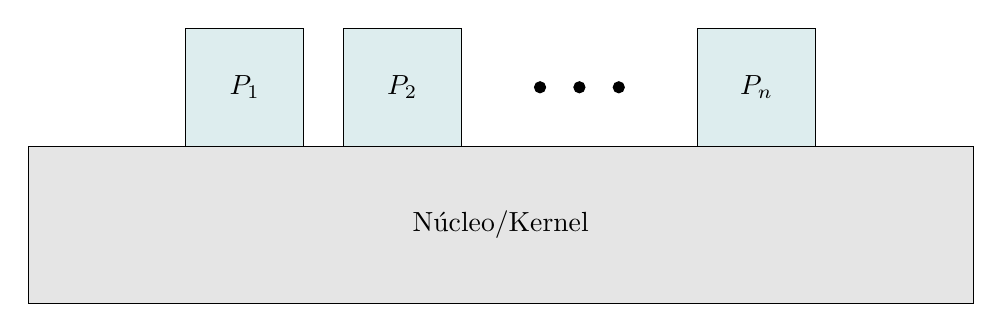
\begin{tikzpicture}
      \draw[fill=gray!20] (-1,0) rectangle node{Núcleo/Kernel} (11,2);
      \foreach \x\t in {2.5/1,4.5/2,9/n} {
        \draw[fill=white!93!green!93!blue] ({\x-1.5},2) rectangle node{$P_\t$} (\x,3.5);
      }
      \foreach \x in {5.5,6,6.5}{
        \filldraw (\x,2.75) circle (2pt);
      }
    \end{tikzpicture}
    \caption{Kernel independiente.}
  \end{subfigure}

  \vspace{0.5cm}

  \begin{subfigure}[c]{\linewidth}
    \centering
    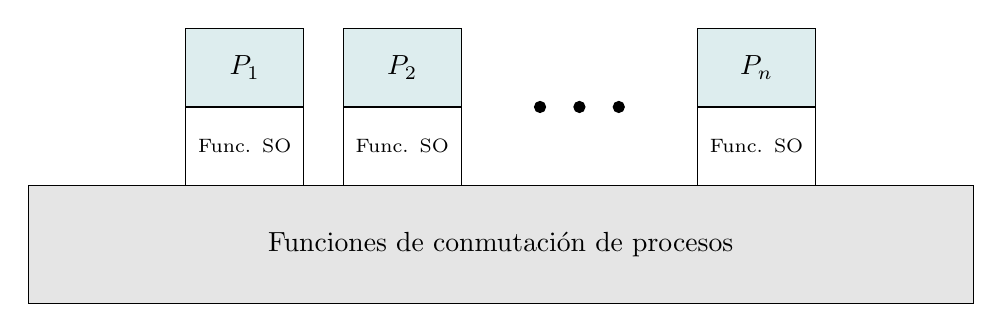
\begin{tikzpicture}
      \draw[fill=gray!20] (-1,0.5) rectangle node{Funciones de conmutación de procesos} (11,2);
      \foreach \x\t in {2.5/1,4.5/2,9/n} {
        \draw ({\x-1.5},2) rectangle node[text width=1.5cm,font=\scriptsize,align=center]{Func. SO} (\x,3);
        \draw[fill=white!93!green!93!blue] ({\x-1.5},3) rectangle node{$P_\t$} (\x,4);
      }
      \foreach \x in {5.5,6,6.5}{
        \filldraw (\x,3) circle (2pt);
      }
    \end{tikzpicture}
    \caption{Funciones del SO se ejecutan dentro del proceso usuario.}
  \end{subfigure}

  \vspace{0.5cm}

  \begin{subfigure}[c]{\linewidth}
    \centering
    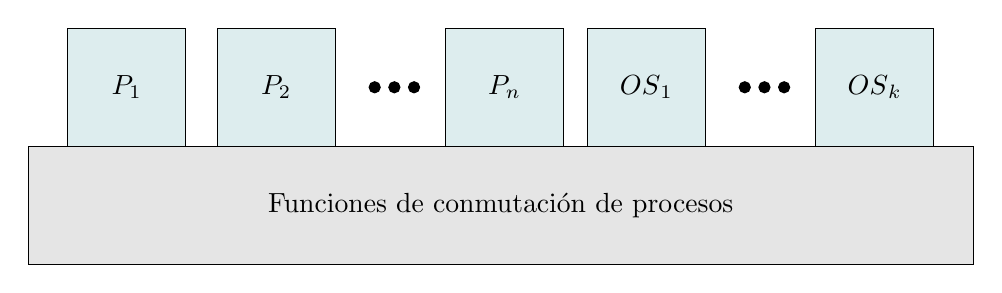
\begin{tikzpicture}
      \draw[fill=gray!20] (-1,0.5) rectangle node{Funciones de conmutación de procesos} (11,2);
      \foreach \x\t in {1/1,2.9/2,5.8/n} {
        \draw[fill=white!93!green!93!blue] ({\x-1.5},2) rectangle node{$P_\t$} (\x,3.5);
      }
      \foreach \x\t in {7.6/1,10.5/k} {
        \draw[fill=white!93!green!93!blue] ({\x-1.5},2) rectangle node{$\text{OS}_\t$} (\x,3.5);
      }
      \foreach \x in {3.4,3.65,3.9}{
        \filldraw (\x,2.75) circle (2pt);
      }
      \foreach \x in {8.1,8.35,8.6}{
        \filldraw (\x,2.75) circle (2pt);
      }
    \end{tikzpicture}
    \caption{Funciones del SO se ejecutan como procesos independientes.}
  \end{subfigure}
  \caption{Relación entre SO y Procesos de usuario.}
\end{figure}

\subsubsection{Núcleo independiente de los procesos (\textit{Nonprocess Kernel})}

En este enfoque, el kernel no pertenece a ningún proceso. Cuando ocurre una interrupción o una llamada al sistema, se guarda el contexto del proceso en ejecución y el control pasa al kernel, el cual utiliza su propia memoria y pila. Una vez completada la operación, el kernel puede reanudar el proceso interrumpido o realizar un cambio de proceso.

La noción de \textit{proceso} se aplica únicamente a los programas de usuario; el kernel se ejecuta como una entidad independiente en \textit{kernel mode}.

\subsubsection{Ejecución dentro de los procesos de usuario}

En este modelo, el código del sistema operativo se ejecuta dentro del contexto del proceso de usuario que invocó un servicio del sistema. El código y los datos del kernel son compartidos por todos los procesos, mientras que cada proceso dispone de una \textit{kernel stack} privada para las ejecuciones en modo kernel.

Cuando ocurre una interrupción, excepción o llamada al sistema, el procesador cambia a \textit{kernel mode}, pero continúa ejecutando el mismo proceso. Por tanto, normalmente solo se produce un mode switch, evitando el costo de un process switch. Solo si el planificador decide ejecutar otro proceso se realiza un cambio de proceso.

\subsubsection{Sistema operativo basado en procesos (\textit{Process-Based OS})}

En este enfoque, el sistema operativo se implementa como un conjunto de procesos del sistema. Cada función importante del kernel se organiza como un proceso independiente, aunque una pequeña parte del código de cambio de contexto puede ejecutarse fuera de cualquier proceso.

Este diseño favorece una arquitectura modular, facilita la implementación de servicios del sistema como procesos independientes y resulta especialmente adecuado para sistemas multiprocesador, donde distintos servicios del sistema operativo pueden ejecutarse en procesadores dedicados.
